\section{Hyperchains Design}
\graphicspath{ {./images/} }

The previous approaches had a lot to offer, but considering their cons it is hard
to scale them reasonably. PoW seems to work well only with big
computational effort being burned and PoS suffers from a huge amount of security
holes that require very complicated algorithms that usually either don't solve
the problem at all or move it further to another layer of abstraction.

Here we present a hybrid strategy that will benefit from the stability of PoW
solutions but will offer the scalability of PoS systems. A Hyperchain is a
special kind of blockchain that sticks to an already existing chain. They are
going to be called child and parent chain respectively\cite{hyperchains}.

The parent chain can be almost any blockchain in the world. In general, we want
to use some big existing PoW based chains (at the time of writing, preferably
Bitcoin or Ethereum, but not limited to) to reuse their burned work to maintain
the stability of the child chain. We would also like to have
PoS-like election system to choose the leaders on the hyperchain. In this case,
however, we have a very reliable – and most important, unpredictable – source
of randomness – the state of the parent chain. The idea is not very new,
though – there is already some research made in this direction\cite{blockchain_random}.

Having this machinery, it seems natural to start a new election each time a
(key)block was mined on the parent chain. The next leader shall be chosen
depending on the hash of that block and selected with chances proportional to
their stake. The selection algorithm is abstract over this document – it is
up to the hyperchain to define the details.

\begin{figure}[h]
	\caption{Component Diagram}
	\centering
	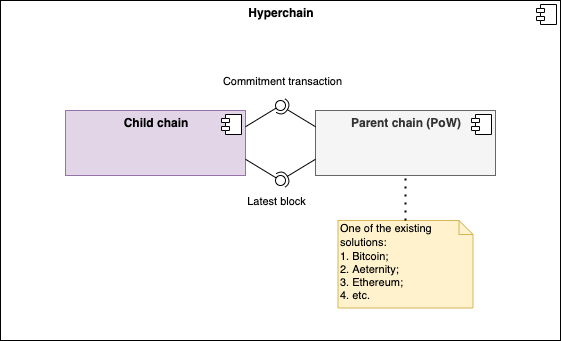
\includegraphics[scale=0.5]{hyperchain_component}
\end{figure}

We define a group of leadership candidates called "delegates." Each delegate
needs to express their will in participation in the election for the upcoming
generation by publishing a commitment transaction onto the parent chain. It is
important to make it clear what is their point of view on the child chain and
over which block they are going to compete.
Therefore the commitment must consist of:
\begin{itemize}
\item The subject of delegation on the child chain
\item The block over the delegate is going to build
\item Signature of the delegate from the child chain
\end{itemize}

One of the important concepts of the commitment idea is to be able to rely on
the parent chain's stability. We want to treat it as a rigid skeleton
of the hyperchain, which can be achieved by proper block hash linking. The
elected leader will be required to publish a key block on the child chain with a
cryptographic proof (referencing the parent) of their right to lead the
upcoming generation and publish microblocks.

One dilemma that rises at this point is whether should the commitment reference
the latest keyblock or the microblock of the child chain. Referencing microblock
on the first sight looks more transparent, but we believe that it would
lead to massive forking (especially when some peers wouldn't receive all of the
blocks). The problem with referencing keyblock is that the next leader could
steal the transactions and post them in their microblocks. This, however, can be
faced with a smarter feeing strategy: instead of giving the full fee to the
miner, we can split it up and give the bigger part to the next leader that did
include the previous leader's microblocks in their continuation of the history,
as it happens in the BitcoinNG\cite{incentive_bcng}.
After getting elected, the new leader posts a keyblock on the child chain that
references the point on the parent, which proves their right to lead the
generation. Besides that, they need to reference the microblock from the previous
generation they want to mine on.


\begin{figure}[h]
	\caption{Hyperchains Design}
	\centering
	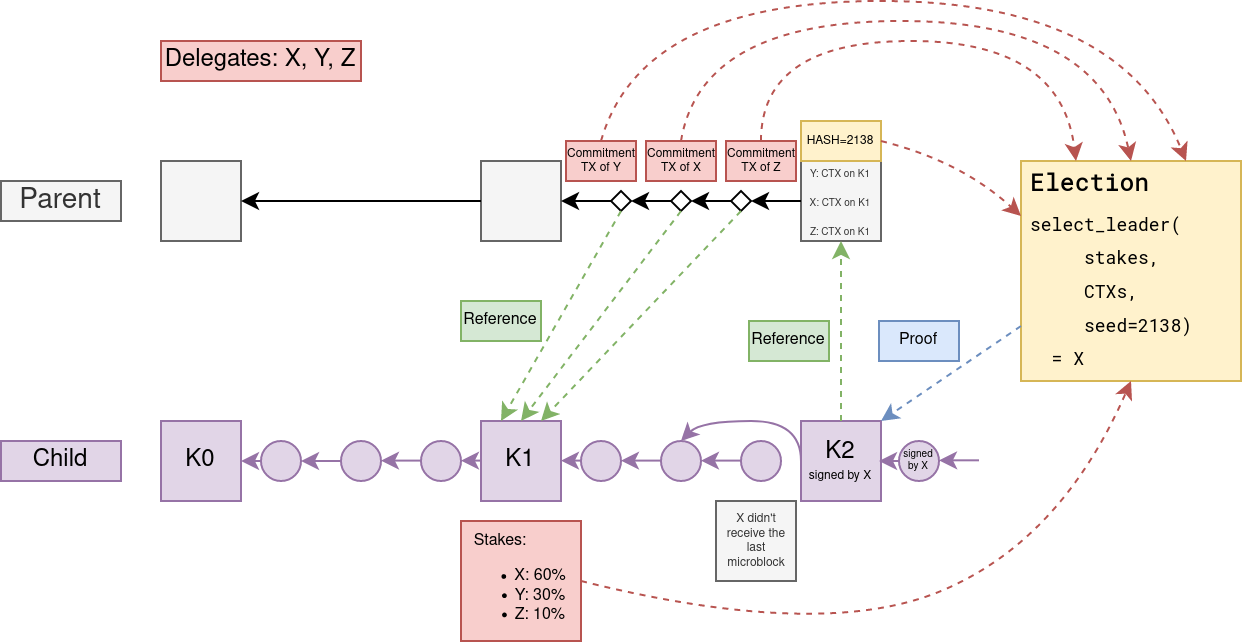
\includegraphics[scale=0.3]{hyperchains_design}
\end{figure}
